\documentclass[11pt,a4paper]{report}

\usepackage[utf8]{inputenc} % File encoding, you should try to stick to utf8.
\usepackage{microtype} % Improve typesetting for pdflatex
\usepackage[parfill]{parskip} % Empty line before paragraphs
\usepackage{csquotes}
\usepackage{hyperref} % Make URLs, page numbers, section references clickable
\usepackage{mathtools}
\usepackage{minted} % For source code highlighting (requires python and pygments)
\usepackage{graphicx}
\usepackage{textcomp} % For copyright symbol and such
\usepackage{wallpaper} % To create the coverpage
\usepackage[english]{babel}
\usepackage[style=ieee, backend=biber]{biblatex}

\addbibresource{bibliography.bib}

% Change chapter style to be similar as sections but larger
\usepackage{titlesec}
\titleformat{\chapter}{\Huge\bfseries}{\thechapter}{20pt}{}

\begin{document}
\pagenumbering{gobble} % Don't show any page numbers
\hypersetup{pageanchor=false, % Deactivate links to page numbers
            linktoc=all} % Make page numbers in TOC clickable

% Title page
\begin{titlepage}
\ThisULCornerWallPaper{1}{resources/frontpage.pdf}
\null
\vfill
\centering
    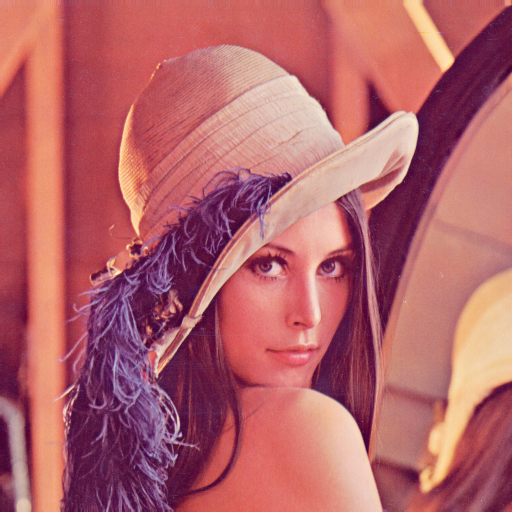
\includegraphics[width=0.9\textwidth]{resources/Lena.png}

\begin{flushleft}
{\Huge Predictive-Reactive Auto-Scaling for Elastic Web Applications}\\[.5cm]
\emph{
    \Large Master of Science Thesis in \\
    Computer Science: Algorithms, Languages and Logic
}\\[.5cm]
{\Large MATTIAS APPELGREN}\\[.5cm]
{
    \Large Department of Computer Science \& Engineering \\
    \textsc{Chalmers University of Technology} \\
    Gothenburg, Sweden 2015 \\
}
\end{flushleft}
\end{titlepage}


% Copyright page
The Author grants to Chalmers University of Technology and University of Gothenburg the non-exclusive right to publish the Work electronically and in a non-commercial purpose make it accessible on the Internet.

The Author warrants that he/she is the author to the Work, and warrants that the Work does not contain text, pictures or other material that violates copyright law.

The Author shall, when transferring the rights of the Work to a third party (for example a publisher or a company), acknowledge the third party about this agreement.  If the Author has signed a copyright agreement with a third party regarding the Work, the Author warrants hereby that he/she has obtained any necessary permission from this third party to let Chalmers University of Technology and University of Gothenburg store the Work electronically and make it accessible on the Internet.\\[.3cm]

Predictive-Reactive Auto-Scaling for Elastic Web Applications\\
MATTIAS APPELGREN\\[.2cm]

\textcopyright MATTIAS APPELGREN, June 2015.\\[.2cm]

Examiner: XXXXXX YYYYYYYY\\
Supervisor: XXXXXX YYYYYYYY\\[.2cm]

Chalmers University of Technology\\
Department of Computer Science and Engineering\\
SE-412 96 Gothenburg\\
Sweden\\
Telephone: +46 (0)31-772 1000\\[.3cm]

Cover: An image representing the thesis.\\[.3cm]

Department of Computer Science and Engineering\\
Gothenburg, Sweden. June 2015.

\clearpage

% Abstract
\begin{abstract}
Lorem ipsum dolor sit amet, consectetur adipisicing elit, sed do eiusmod tempor incididunt ut labore et dolore magna aliqua. Ut enim ad minim veniam, quis nostrud exercitation ullamco laboris nisi ut aliquip ex ea commodo consequat. Duis aute irure dolor in reprehenderit in voluptate velit esse cillum dolore eu fugiat nulla pariatur. Excepteur sint occaecat cupidatat non proident, sunt in culpa qui officia deserunt mollit anim id est laborum.

Lorem ipsum dolor sit amet, consectetur adipiscing elit. Donec viverra gravida adipiscing. Morbi vitae dui eu leo dapibus venenatis quis laoreet augue. Proin sem nunc, lobortis sed gravida id, iaculis id justo. Sed convallis, mauris vel mattis posuere, tortor quam molestie sem, vel feugiat risus dolor sit amet purus. Nulla facilisi. Duis ac velit non tortor malesuada pellentesque vitae vitae erat. Aliquam dapibus porta lorem lacinia vestibulum. Nulla convallis venenatis euismod. Suspendisse adipiscing lacus id nisi hendrerit dapibus. Sed quam diam, pretium vel accumsan vel, pulvinar et odio. Nulla facilisis ullamcorper metus non suscipit. Aliquam nec augue odio. In hac habitasse platea dictumst. Nulla facilisi. Pellentesque habitant morbi tristique senectus et netus et malesuada fames ac turpis egestas. Maecenas consequat mattis metus, in imperdiet purus suscipit eu. Mauris velit lorem, pharetra nec vehicula cursus, vulputate sit amet dui. Nam sed eros magna, quis molestie urna.

\end{abstract}

% Acknowledgements
\renewcommand{\abstractname}{Acknowledgements}
\begin{abstract}
Lorem ipsum dolor sit amet, consectetur adipisicing elit, sed do eiusmod tempor incididunt ut labore et dolore magna aliqua. Ut enim ad minim veniam, quis nostrud exercitation ullamco laboris nisi ut aliquip ex ea commodo consequat. Duis aute irure dolor in reprehenderit in voluptate velit esse cillum dolore eu fugiat nulla pariatur. Excepteur sint occaecat cupidatat non proident, sunt in culpa qui officia deserunt mollit anim id est laborum. \\[1cm]

\hfill The Authors, Location 11/9/11

\end{abstract}

% Table of contents
\tableofcontents
\clearpage

% Thesis starts here
\hypersetup{pageanchor=true} % Activate links to page numbers
\pagenumbering{arabic} % Start showing page numbers (from 1)

\chapter{Introduction}
Do not forget to read section~\ref{sec:motivation}. Lorem ipsum dolor sit amet \cite{matlab:ode}, consectetur adipiscing elit. Donec viverra gravida adipiscing \cite{paper:A}. Morbi vitae dui eu leo dapibus venenatis quis laoreet augue. Proin sem nunc, lobortis sed gravida id, iaculis id justo. Sed convallis, mauris vel mattis posuere, tortor quam molestie sem, vel feugiat risus dolor sit amet purus. Nulla facilisi. Duis ac velit non tortor malesuada pellentesque vitae vitae erat. Aliquam dapibus porta lorem lacinia vestibulum. Nulla convallis venenatis euismod. Suspendisse adipiscing lacus id nisi hendrerit dapibus. Sed quam diam, pretium vel accumsan vel, pulvinar et odio. Nulla facilisis ullamcorper metus non suscipit. Aliquam nec augue odio. In hac habitasse platea dictumst. Nulla facilisi. Pellentesque habitant morbi tristique senectus et netus et malesuada fames ac turpis egestas. Maecenas consequat mattis metus, in imperdiet purus suscipit eu. Mauris velit lorem, pharetra nec vehicula cursus, vulputate sit amet dui. Nam sed eros magna, quis molestie urna.
\section{Motivation}\label{sec:motivation}
Just a math thing \( \forall x \in X \) and another one:
\[ \alpha^2 + \beta^2 = \gamma^2 \]

Lorem ipsum dolor sit amet, consectetur adipiscing elit. Donec viverra gravida adipiscing. Morbi vitae dui eu leo dapibus venenatis quis laoreet augue. Proin sem nunc, lobortis sed gravida id, iaculis id justo. Sed convallis, mauris vel mattis posuere, tortor quam molestie sem, vel feugiat risus dolor sit amet purus. Nulla facilisi. Duis ac velit non tortor malesuada pellentesque vitae vitae erat
\begin{table}[h]
  \begin{center}
    \begin{tabular}{| l c r |}
    \hline
    1 & 2 & 3 \\
    4 & 5 & 6 \\
    7 & 8 & 9 \\
    \hline
    \end{tabular}
  \end{center}
  \caption{A simple table}
  \label{tab:simple1}
\end{table}

\autoref{tab:simple1} is a very simple example. Lorem ipsum dolor sit amet, consectetur adipiscing elit. Donec viverra gravida adipiscing. Morbi vitae dui eu leo dapibus venenatis quis laoreet augue. Proin sem nunc, lobortis sed gravida id, iaculis id justo. Sed convallis, mauris vel mattis posuere, tortor quam molestie sem, vel feugiat risus dolor sit amet purus. Nulla facilisi. Duis ac velit non tortor malesuada pellentesque vitae vitae erat. Aliquam dapibus porta lorem lacinia vestibulum. Nulla convallis venenatis euismod. Suspendisse adipiscing lacus id nisi hendrerit dapibus. Sed quam diam, pretium vel accumsan vel, pulvinar et odio. Nulla facilisis ullamcorper metus non suscipit. Aliquam nec augue odio. In hac habitasse platea dictumst. Nulla facilisi. Pellentesque habitant morbi tristique senectus et netus et malesuada fames ac turpis egestas. Maecenas consequat mattis metus, in imperdiet purus suscipit eu. Mauris velit lorem, pharetra nec vehicula cursus, vulputate sit amet dui. Nam sed eros magna, quis molestie urna.
\begin{figure}[h]
    \centering
        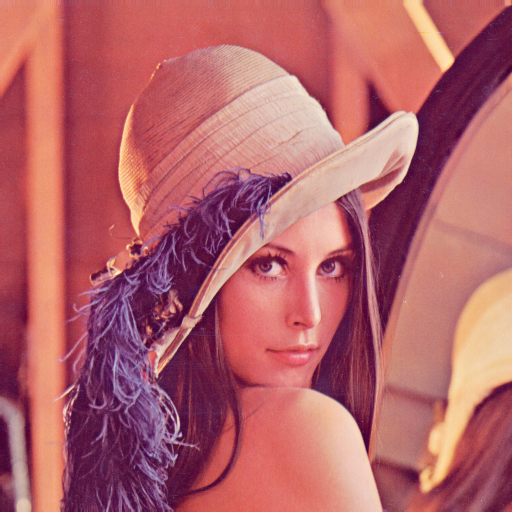
\includegraphics[width=0.8\textwidth]{resources/Lena.png}
    \caption{This is an image}
    \label{fig:lena}
\end{figure}

Figure \ref{fig:lena} shows a picture. Lorem ipsum dolor sit amet, consectetur adipiscing elit. Donec viverra gravida adipiscing. Morbi vitae dui eu leo dapibus venenatis quis laoreet augue. Proin sem nunc, lobortis sed gravida id, iaculis id justo. Sed convallis, mauris vel mattis posuere, tortor quam molestie sem, vel feugiat risus dolor sit amet purus. Nulla facilisi. Duis ac velit non tortor malesuada pellentesque vitae vitae erat. Aliquam dapibus porta lorem lacinia vestibulum. Nulla convallis venenatis euismod. Suspendisse adipiscing lacus id nisi hendrerit dapibus. Sed quam diam, pretium vel accumsan vel, pulvinar et odio. Nulla facilisis ullamcorper metus non suscipit. Aliquam nec augue odio. In hac habitasse platea dictumst. Nulla facilisi. Pellentesque habitant morbi tristique senectus et netus et malesuada fames ac turpis egestas. Maecenas consequat mattis metus, in imperdiet purus suscipit eu. Mauris velit lorem, pharetra nec vehicula cursus, vulputate sit amet dui. Nam sed eros magna, quis molestie urna.
\begin{minted}[]{haskell}
f 0 = 0
f 1 = 1
f a = f (a-1) + f (a-1)
\end{minted}


% Bibliography
\nocite{*} % Add everything from the bibliography TODO: Remove
\printbibliography[heading=bibintoc]

% Appendices
\appendix
\chapter{Data}
Data goes here


\end{document}
